\documentclass[tikz]{standalone}
\usepackage{amsmath}
\definecolor{pagebg}{HTML}{171D2B}
\definecolor{aksen}{HTML}{F7B538}
\pagecolor{pagebg}
\color{white}
\begin{document}
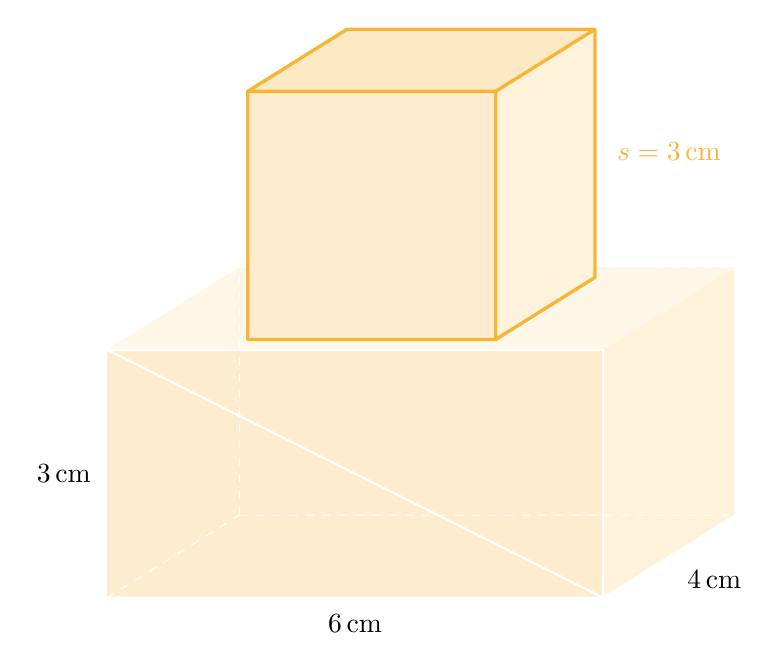
\begin{tikzpicture}[scale=1.05, line join=round]
% Proyeksi: x' = x + 0.4z ; y' = y + 0.25z  (1 unit = 1 cm)
% BALOK p=6 (x), t=3 (y), l=4 (z)
\coordinate (A) at (0,0);
\coordinate (B) at (6,0);
\coordinate (C) at (7.6,1.0);
\coordinate (D) at (1.6,1.0);
\coordinate (E) at (0,3);
\coordinate (F) at (6,3);
\coordinate (G) at (7.6,4.0);
\coordinate (H) at (1.6,4.0);
% KUBUS s=3 di atas balok: x 1.5..4.5, z 0.5..3.5, y 3..6
\coordinate (K1) at (1.7,3.125);
\coordinate (K2) at (4.7,3.125);
\coordinate (K3) at (5.9,3.875);
\coordinate (K4) at (2.9,3.875);
\coordinate (K5) at (1.7,6.125);
\coordinate (K6) at (4.7,6.125);
\coordinate (K7) at (5.9,6.875);
\coordinate (K8) at (2.9,6.875);
% sisi balok
\fill[aksen!12] (E) -- (F) -- (G) -- (H) -- cycle;   % alas atas
\fill[aksen!25] (A) -- (B) -- (F) -- (E) -- cycle;   % depan
\fill[aksen!18] (B) -- (C) -- (G) -- (F) -- cycle;   % kanan
% rusuk tersembunyi balok
\draw[white!45,dashed] (A) -- (D) (D) -- (H) (D) -- (C) (H) -- (G);
% rusuk balok terlihat
\draw[white,thick] (A)--(B)--(C)--(G) (B)--(F)--(E)--cycle (E)--(F);
% kubus menutupi sebagian alas atas
\fill[aksen!25] (K1) -- (K2) -- (K6) -- (K5) -- cycle;
\fill[aksen!18] (K2) -- (K3) -- (K7) -- (K6) -- cycle;
\fill[aksen!30] (K5) -- (K6) -- (K7) -- (K8) -- cycle;
\draw[aksen,very thick] (K1)--(K2)--(K3)--(K7)--(K8)--(K5)--cycle;
\draw[aksen,very thick] (K5)--(K6)--(K7) (K6)--(K2);
% label
\node[below] at (3,-0.08) {$6\,\text{cm}$};
\node[below right] at (6.9,0.45) {$4\,\text{cm}$};
\node[left] at (-0.08,1.5) {$3\,\text{cm}$};
\node[right,aksen] at (6.05,5.4) {$s=3\,\text{cm}$};
\end{tikzpicture}
\end{document}